\subsection{Правило Лопиталя (для $\frac{0}{0}$ и $\frac{\infty}{\infty}$). Примеры \href{https://youtu.be/au9-34CerJM?t=278}{\Walley}}

\begin{theorem-non} 
    Правило Лопиталя для $\frac{0}{0}$

    Пусть 
    \begin{itemize}
        \item $-\infty \leq a < b \leq +\infty$
        \item $f$ и $g$ дифференцируемы на $(a, b)$
        \item $g'(x) \neq 0 \quad \forall x \in (a, b)$
        \item $\lim\limits_{x \rightarrow b-} f(x) = \lim\limits_{x \rightarrow b-} g(x) = 0$
    \end{itemize}
    Тогда если $\lim\limits_{x \rightarrow b-}\frac{f'(x)}{g'(x)} = l \in \overline{\mathbb{R}}$, 
    то $\lim\limits_{x \rightarrow b-}\frac{f(x)}{g(x)} = l$
\end{theorem-non}
\begin{proof}
    Проверяем определение по Гейне. Берем последовательность $x_n \longrightarrow b$. Можно считать, что $x_n$ строго возрастает, 
    потому что предел не меняется от перестановки членов последовательности и её прорежения.

    Надо проверить, что $\frac{f(x_n)}{g(x_n)} \longrightarrow l$.

    Тогда по теореме Штольца посмотрим на $\frac{f(x_{n+1}) - f(x_n)}{g(x_{n+1}) - g(x_n)}$. Чтобы применилась т. Штольца, надо:
    \begin{itemize}
        \item числитель и знаменатель стремятся к 0 ($\lim\limits_{x \rightarrow b-} f(x) = \lim\limits_{x \rightarrow b-} g(x) = 0$)
        \item знаменатель был строго монотонен ($g'(x) \neq 0 \quad \forall x \in (a, b)$, 
        поэтому по следствию т. Дарбу $g$ строго монотонна, последовательность аргументов тоже строго монотонна, тогда последовательность значений тоже строго монотонна)
    \end{itemize}

    $\frac{f(x_{n+1}) - f(x_n)}{g(x_{n+1}) - g(x_n)} = \frac{f'(c_n)}{g'(c_n)}$ для некоторого $c_n \in (x_n, x_{n+1})$ (по теореме Коши)
    
    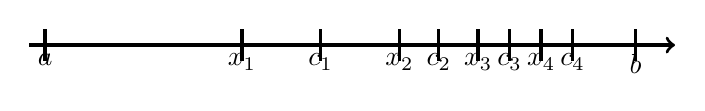
\begin{tikzpicture}[mydrawstyle/.style={draw=black, very thick}, x=1mm, y=1mm, z=1mm]
        \draw[mydrawstyle, ->](-2,30)--(80,30);
        \draw[mydrawstyle](0,28)--(0,32) node[below=5]{$a$};
        \draw[mydrawstyle](25,28)--(25,32) node[below=5]{$x_1$};
        \draw[mydrawstyle](35,28)--(35,32) node[below=5]{$c_1$};
        \draw[mydrawstyle](45,28)--(45,32) node[below=5]{$x_2$};
        \draw[mydrawstyle](50,28)--(50,32) node[below=5]{$c_2$};
        \draw[mydrawstyle](55,28)--(55,32) node[below=5]{$x_3$};
        \draw[mydrawstyle](59,28)--(59,32) node[below=5]{$c_3$};
        \draw[mydrawstyle](63,28)--(63,32) node[below=5]{$x_4$};
        \draw[mydrawstyle](67,28)--(67,32) node[below=5]{$c_4$};
        \draw[mydrawstyle](75,28)--(75,32) node[below=5]{$b$};
    \end{tikzpicture}

    Тогда $c_n \longrightarrow b$  и строго возрастают.

    $\lim c_n = b \Longrightarrow \lim \frac{f'(c_n)}{g'(c_n)} = l$ (по определению $\lim\limits_{x \rightarrow b-}\frac{f(x)}{g(x)}$ по Гейне)

    $\Longrightarrow \lim \frac{f(x_{n+1}) - f(x_n)}{g(x_{n+1}) - g(x_n)} = l \Longrightarrow \lim\limits_{x \rightarrow b-}\frac{f(x)}{g(x)} = l$ (по т. Штольца)

\end{proof}

\begin{theorem-non}
    Правило Лопиталя для $\frac{\infty}{\infty}$

    Пусть 
    \begin{itemize}
        \item $-\infty \leq a < b \leq +\infty$
        \item $f$ и $g$ дифференцируемы на $(a, b)$
        \item $g'(x) \neq 0 \quad \forall x \in (a, b)$
        \item $\lim\limits_{x \rightarrow b-} g(x) = +\infty$
    \end{itemize}
    Тогда если $\lim\limits_{x \rightarrow b-}\frac{f'(x)}{g'(x)} = l \in \overline{\mathbb{R}}$, 
    то $\lim\limits_{x \rightarrow b-}\frac{f(x)}{g(x)} = l$

\end{theorem-non}
\begin{proof}
    Доказательство такое же, но в последней строке ссылаемся на вторую версию т. Штольца. 
\end{proof}

\textbf{Примеры:}

\begin{enumerate}
    \item $\lim\limits_{x \rightarrow +\infty} \frac{\ln x}{x^p} = 0$ при $p > 0$ (проверьте Лопиталем сами)
    \item $\lim\limits_{x \rightarrow +\infty} \frac{x^p}{a^x} = 0$ при $a > 1, \ p \in \mathbb{R}$
    \begin{proof}
        При $p \leqslant 0$ очевидно.

        $\frac{x^p}{a^x} = \frac{px^{p-1}}{a^x \ln a} = \frac{p}{\ln a} \cdot \frac{x^{p-1}}{a^x} \longrightarrow 0$ очевидно при $p \leqslant 1$

        и так далее дифференцируем.
    \end{proof}
    \item $\lim\limits_{x \rightarrow 0+} x^x = 1$
    \begin{proof}
        Прологарифмируем: $\lim\limits_{x \rightarrow 0+} x \ln x = 0$ 
        (если это поймем, то применим к обеим сторонам экспоненту, так как $\exp(\lim \dots)) = \lim \exp \dots$)

        $\lim\limits_{x \rightarrow 0+} x \ln x = \lim\limits_{x \rightarrow 0+} \frac{\ln x}{1/x} = \lim\limits_{x \rightarrow 0+} \frac{1/x}{-1/x^2} = -x \longrightarrow 0$ (по правилу Лопиталя)
    \end{proof}
\end{enumerate}

